\section{Strings: Algo así como una pregunta para saber usar el ciclo for}

Los teléfonos incorporaron una entretenida manera de escribir mensajes de texto usando números, en este caso, se debía repetir el número tantas veces según la posición de la letra que quisiera escribir. Por ejemplo, para escribir CIAC la secuencia de números es 222 444 2 222. Considere que la tecla 0 genera un espacio.

\begin{figure}[h]
    \centering
    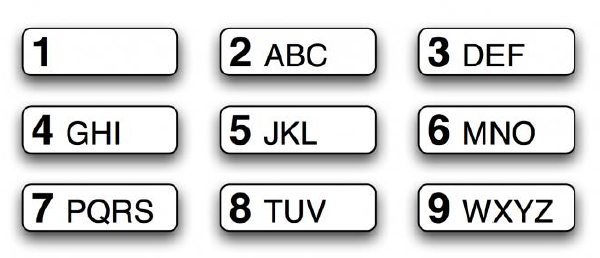
\includegraphics{Guia/teclado.png}
\end{figure}

\begin{itemize}
    \item Su desafío será escribir el código para que un programa pida al usuario una serie de números separados por espacio y que imprima por pantalla el mensaje en letras.
\begin{lstlisting}[style=consola]
Ingrese mensaje: [*33 7777 8 88 3 444 2 777 0 222 666 66 0 6 444 4 88 33 555 
0 33 7777 0 22 2 222 2 66*]
El mensaje es: ESTUDIAR CON MIGUEL ES BACAN
\end{lstlisting}
    \item Cree una función \texttt{traducir\_letra(letra)} que reciba un string con una letra en mayúscula (o un espacio) e indique el número a presionar las veces que sea necesario.
\begin{lstlisting}[style=consola]
>>> [*traducir_letra('F')*]
'333'
\end{lstlisting}
    \item Implemente la función anterior con un programa que pida al usuario un mensaje a traducir e imprima por pantalla la seguidilla de números a presionar en el teclado de celular.
\begin{lstlisting}[style=consola]
Ingrese mensaje: [*VENIR A CIAC ES LA CUMBIA*]
888 33 66 444 777 0 2 0 222 444 2 222 0 33 7777 0 555 2 0 222 88 6 22 444 2
\end{lstlisting}
\end{itemize}